\clearpage
\section*{Annotatsioon - Praktilise küberkaitse e-kursus
süsteemiadministraatoritele}
\label{kokkuvõte}
\thispagestyle{empty}
\begin{Huge}
Hands-On E-learning Course on Cyber Defence for System Administrators.\par
\end{Huge}

\selectlanguage{estonian}
Käesolev magistritöö käsitleb praktilise küberkaitse e-kursuse loomist IT süsteemide administreerijatele. Põhiline töös lahendatav probleem on turvateadlike IT taristu teenuste administraatorite vähesus. Probleemi lahendamiseks loodi praktiline laboritöödel põhinev kursus, mis on kasutatav nii tasemeõppes kui ka täiendusõppes.

Kursuse koostamisel kasutati \gls{ADDIE} (\emph{Analysis, Design, Development, Implementation, Evaluation}) metoodikat, mis sobib e-kursuse loomiseks. Loodud e-kursus erineb teistest Eestis kasutusel olevatest kursustest, kuna on loodud sihtgrupile ja fookusega IT taristu teenuste kaitsele.

Kasutatud \gls{ADDIE} mudel koosneb viiest etapist: analüüsi etapp, kavandamise etapp, väljatöötamise etapp, läbiviimise etapp, hindamise etapp  Joonis~\ref{figure:addie mudel} \citep{website:addie}.


\begin{figure}[H]
 \centering 
 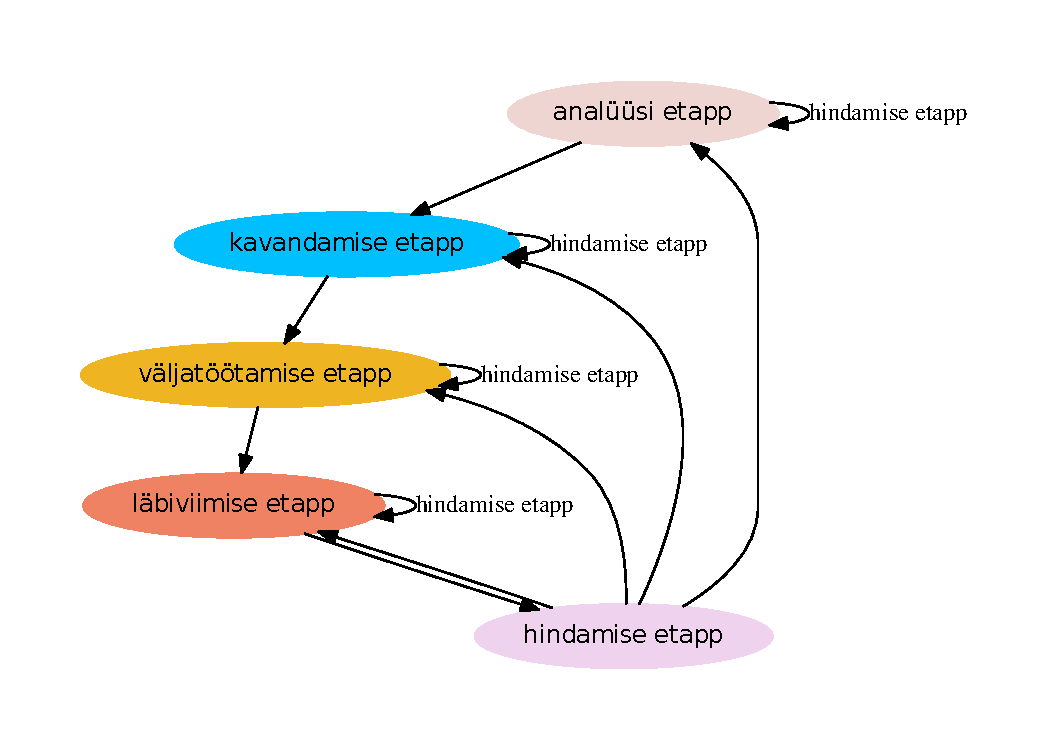
\includegraphics[width=0.6\textwidth]{addie_model_eesti.pdf}
 \rule{35em}{0.5pt} 
 \caption{ADDIE mudel} 
 \label{figure:addie mudel} 
\end{figure}
 Joonis~\ref{figure:the addie model} \citep{website:addie}.



Suurendamaks kaitsele orienteeritud kursuse põnevust tudengite seas on kasutusel medalite süsteem ja edetabel, mis toob kaasa võistlusmomendi. Kursusel kasutatakse probleemipõhist õpet praktiliste ülesannete puhul, koostööl põhinevat õpet rühmatöö vormis laboriaruannete  koostamisel ja kogukonnapõhist õpet abistavate ja selgitavate õppematerjalide loomiseks.

Töö tulemusena valmis uus väljundipõhine kursus mahuga 6 EAP-d (32h loenguid, 46h praktilist tööd, 78h iseseisvat tööd), mida piloteeriti Eesti Infotehnoloogia Kolledžis tasemeõppes ja täiendusõppes. %Kursus koosneb loengutest, nende videosalvestustest, enese ja eelduste testidest, praktilistest, probleemile orienteeritud laboritöödest ja interaktiivsetest testidest.

Kursuse tagasiside on positiivne ja kursuse tulemusena paraneb tudengite ja ettevõtete süsteemide administreerijate turvateadlikus.
% Kursuse loomisel kasutati erinevate ettappide kvaliteedi hindamiseks teiste õppejõudude ja tudengite abi.

Autori roll seisnes nõuete ja õpiväljundite loomises, laboritööde ja loengumaterjalide koostamises koostöös teiste õppejõududega (panus >90\%) ja kursuse piloteerimises nii taseme- kui täiendõppes.
